% --------------------
  \chapter{Diseño}
% --------------------
\label{C:diseño}

Para la etapa de diseño, se dividirá en tres partes.

\begin{itemize}
\item La primera, será el diseño eléctrico del carrito omnidireccional, con los componentes necesarios para funcionar.
\item La segunda es el diseño del código para el carrito omnidireccional, encargado del control de los motores y la odometría de las ruedas.
\item Por último, se hablará del diseño necesario del lado de la computadora principal, para lograr la navegación y el mapeo.
\end{itemize}

\newpage

\section{Carrito omnidireccional}
Para la primera etapa, se utilizará el esquema básico presentado en la figura \ref{F:diagrama}. Se requiere de un sistema que pueda controlar los motores, y además llevar control de la odometría de las ruedas. Además se deberá incorporar el sensor de profundidad en el carrito omnidireccional.

\begin{figure}[H]
\centering
\includegraphics[scale=0.6]{imagenes/diagrama_diseno.png}
\caption{Diagrama básico de la implementación de la parte elétrica del carrito omnidireccional. Autoría propia.}
\label{F:diagrama}
\end{figure}

\subsection{Motores}

Empezando por los \textbf{motores}, se utilizarán motores DC Actobotics 638276. La hoja de fabricante con los datos en la sección de los apéndices. Además, en la tabla \ref{T:actobotics} se muestra la información más relevante de los motores a utilizar, como por ejemplo el consumo máximo, la tensión de trabajo, y la relación de los engranes.

\begin{table}[H]
\caption{Información más relevante de los motores Actobotics, a ser utilizados. Autoría propia.}
\begin{tabular}{|l|l|}
\hline
Especificación                & Valor         \\ \hline
Voltage de operación          & 6-12 VDC      \\ \hline
Corriente máxima de operación & 0.53 A        \\ \hline
Velocidad máxima sin carga    & 118 $\pm$ 12 rpm \\ \hline
Corriente máxima detenido     & 20 A          \\ \hline
Razón de los engranes         & 1/71          \\ \hline
Clicks del encoder por revolución & 3408      \\ \hline
\end{tabular}
\label{T:actobotics}
\end{table}

Se utilizarán cuatro motores, uno para cada rueda, conectados a ruedas mecanum genericas, de 6mm de diámetro. Estas son ruedas omnidireccionales con rodillos a un ángulo de $\alpha = 45^\circ$.

\subsection{Controladores}

En lo que concierne a los \textbf{controladores} de los motores, no se diseñarán, puesto que se utilizarán controladores comerciales de marca IonMotion Roboclaw. En específico, se utilizará el modelo Roboclaw 2x15A. En el cuadro \ref{T:roboclaw} se resumen los datos más importantes de este controlador.

\begin{table}[H]
\caption{Información más relevante de los controladores Roboclaw 2x15A. Autoría propia.}
\begin{tabular}{|l|l|}
\hline
Especificación                      & Valor          \\ \hline
Tensión de la batería principal     & 6-34 VDC       \\ \hline
Tensión de la batería lógica        & 6-34 VDC       \\ \hline
Bits de los contadores para encoder & 32 bits        \\ \hline
Velocidad máxima sin carga          & 118 +- 12 rpm  \\ \hline
R232 Baud Rate                      & 460,800 Bits/s \\ \hline
Tensión de I/O                      & 3.3 VDC        \\ \hline
\end{tabular}
\label{T:roboclaw}
\end{table}

Es importante mencionar, que estos controladores se utilizan para manejar los motores. Pueden manejar hasta dos motores, y son muy versátiles en cuánto a cómo se pueden utilizar. En particular, para este proyecto se usará la comunicación serial que posee el controlador. En la figura \ref{F:roboclaw} se muestran los pines que posee el roboclaw. En específico, los pines S1, y S2 se pueden utilizar como puertos USART para comunicación serial. La tabla \ref{T:pines} muestra las funcionalidades que pueden cumplir cada pin.

\begin{figure}[H]
\centering
\includegraphics[scale=0.5]{imagenes/roboclaw.png}
\caption{Muestra de los pines de un Roboclaw 2x15A fabricado por IonMotion. Tomado del manual del fabricante.}
\label{F:roboclaw}
\end{figure}

\begin{table}[H]
\centering
\caption{Tabla con las funciones de los pines en un Roboclaw 2x15A fabricado por IonMotion. Tomado del manual del fabricante.}
\includegraphics[scale=0.7]{imagenes/pines.png}
\label{T:pines}
\end{table}

Se utilizará una frecuencia de 115200 en la transmisión serial, ya que es la más alta soportada por el dispositivo. En el modo llamado ``Packet Serial'', el cuál funciona mediante el protocolo RS-232 para controlar la dirección y velocidad de cada uno de los motores.

El fabricante da ejemplo de código que se puede utilizar para enviar comandos, y especifica el protocola utilizado en el manual de usuario. Todas las instrucciones utilizan un checksum crc16bit para verificación de las intrucciones.

\subsection{Microcontrolador}

Siguiendo el esquema de la figura \ref{F:diagrama}, los controladores Roboclaw van conectados al \textbf{microcontrolador} STM32F411. La principal función de este microcontrolador será llevar cuenta de la odometría de cada una de las ruedas, y del robot como tal. Además, este aceptará instrucciones por USB del Raspberry Pi, de movimiento en el formato $(V_X, V_Y, W_Z)$ y enviará información de vuelta de la odometría del robot en el formato $(X_X, X_Y, \alpha_Z)$. También enviará instrucciones de movimiento a los dos controladores Roboclaw, y controlará la velocidad de cada motor por medio de un PID, en lazo cerrado con la información del encoder como entrada.

El esquema mostrado en la figura \ref{F:diagrama_stm} muestra en resumen lo que se explicó anteriormente.

\begin{figure}[H]
\centering
\includegraphics[scale=0.5]{imagenes/microcontrolador_diagrama.png}
\caption{Diagrama de las funciones que debe realizar el microcontrolado STM32F411. Autoría propia.}
\label{F:diagrama_stm}
\end{figure}

Es importante notar, que la programación del microcontrolador se realizará mediante las liberías libopencm3 y libopencm3-plus, las cuáles permiten escribir el código en el lenguaje de programación C. Además, el microcontrolador posee las funciones para leer los encoders directamente, puesto que posee timers que se pueden configurar en un modo para leer codificadores de cuadratura.

Información sobre el uso de encoders de cuadratura en el stm se puede encontrar en apéndice correspondiente.

\subsection{Diagrama eléctrico}

Finalmente, un diagrama de las conexiones eléctricas se puede encontrar en la figura \ref{F:conexiones}. En este diagrama se incluye la información de los pines pertinentes en cada dispositivo.

\begin{figure}[h!]
\centering
\includegraphics[scale=0.63]{imagenes/diagrama_electrico.png}
\caption{Diagrama de las conexiones eléctricas entre los dispositivos. Autoría propia.}
\label{F:conexiones}
\end{figure}

\section{Código del stm32f411}
Para el diseño del código, se debe considerar el hardware que se tiene y las funciones que este permite. A continuación se listarán las funciones que debe cumplir el código por escribir:

\begin{enumerate}
\item Librería de comunicación hacia el Roboclaw. Comandos básicos de prueba, como leer firmware, leer información de la batería, y enviar comandos de velocidad.
\item Escribir una función que sea llamada por medio de interrupciones de hardware, cada cierto tiempo constante, para llevar control de la velocidad de cada encoder, y la posición del encoder.
\item Diseñar una función que controle la velocidad de cada rueda, por medio de un control PID discreto.
\item Diseñar un protocolo de comunicación que permita recibir comandos de velocidad del Raspberry Pi, y enviar información de la odometría del robot al mismo.
\item Escribir la función que realice el cálculo de la odometría real del robot en cada interrupción por hardware.
\end{enumerate}

\subsection{Librería de comunicación}
Para escribir la librería, el manual de usuario del roboclaw menciona la estructura básica de los diferentes comandos que acepta el Roboclaw. Se implementarán un total de 6 instrucciones para proporcionar el funcionamiento básico del robot. En el apéndice se puede encontrar más información acerca de la estructura de las instrucciones. En particular nos interesan las intrucciones 0, 1, 4, 5, 21 y 24. A continuación se muestra la estructura de las instrucciones a implementar:

\begin{itemize}
\item \textbf{Instrucción 0:} Drive Forward M1. Se utiliza para mover el motor 1 hacia adelante. Tiene valores válidos desde el rango de 0 a 127, donde 127 es velocidad máxima, y 0 completamente detenido. Se manda de la siguiente manera:

Dirección, 0,  Valor, CRC(2 bytes)

\item \textbf{Instrucción 1:} Drive Backwards M1. Se utiliza para mover el motor 1 hacia atrás. Tiene valores válidos desde el rango de 0 a 127, donde 127 es velocidad máxima, y 0 completamente detenido. Se manda de la siguiente manera:

Dirección, 1, Valor, CRC(2 bytes)

Recibe lo siguiente:

0xFF

\item \textbf{Instrucción 4:} Drive Forward M2. Se utiliza para mover el motor 2 hacia adelante. Tiene valores válidos desde el rango de 0 a 127, donde 127 es velocidad máxima, y 0 completamente detenido. Se manda de la siguiente manera:

Dirección, 4,  Valor, CRC(2 bytes)

Recibe lo siguiente:

0xFF

\item \textbf{Instrucción 5:} Drive Backwards M2. Se utiliza para mover el motor 2 hacia atrás. Tiene valores válidos desde el rango de 0 a 127, donde 127 es velocidad máxima, y 0 completamente detenido. Se manda de la siguiente manera:

Dirección, 5, Valor, CRC(2 bytes)

Recibe lo siguiente:

0xFF

\item \textbf{Instrucción 21:} Read Firmware Version. Se utiliza para leer la información de la versión de software que actualmente se encuentra corriente en el controlador. Lo que se envía es bastante sencillo:

Dirección, 21

Recibe algo similar a lo siguiente:

“RoboClaw 10.2A v4.1.11”,10,0, CRC(2 bytes)

\item \textbf{Instrucción 24:} Read Logic Battery Voltage Level. Se utiliza para medir la tensión entre las terminales B+ y B-. La información se encuentra en decenas de voltage, ejemplo: 300 = 30V. A continuación se muestra lo que se debe enviar:

Dirección, 24

Recibe lo siguiente

Valor (2 bytes), CRC (2 bytes)

\end{itemize}

Esta librería se programará en el microcontrolador STM32, para poder enviar mensajes hacia el controlador de los motores. Es importante destacar que el microcontrolador posee soporte para puertos USART. Inclusive, la librería libopencm3 posee un paquete para transimisión a través de estos puertos. Sencillamente se utilizan dos comandos importantes, los cuáles son \textit{usart\_send\_blocking} y \textit{usart\_recv\_blocking}.

Respectivamente mandan y reciben un byte de información a la vez, y los bits de inicio y fin son configurables, al igual que la velocidad de transferencia, la cuál debe coincidir con la velocidad del controlador Roboclaw. Además de estos, existen otros parámetros que se deben configurar para el funcionamiento correcto del puerto de comunicación. La figura \ref{F:usart} muestra un ejemplo de cómo configurar un puerto usart utilzando la librería libopencm3.

\begin{figure}[H]
\centering
\includegraphics[scale=0.5]{imagenes/usart.png}
\caption{Ejemplo de configuración de un puerto USART utilizando la librería libopencm3. Autoría propia.}
\label{F:usart}
\end{figure}

\subsection{Encoder}

Para llevar el conteo de la cantidad de ticks que ha ocasionado un encoder en un timer del stm32f411, se debe leer constantemente el estado de cada timer, y transferir la información a una variable donde se lleve la cuenta de los ticks. Esta lectura debe de ser en intervalos de tiempo constante, para a su vez poder calcular la velocidad del motor.

El microcontrolador stm32f411 posee una función llamada systick, el cuál es un contador que produce una bandera cuando llega al valor de recarga, el cuál puede ser configurado. Esta bandera es utilizada para llamar una subrutina, que ha de ser ejecutada en el momento en que se produce la bandera.

Por lo tanto, se obtienen interrupciones en intervalos contantes, que son producidas cada cierta cantidad de ciclos de reloj. La figura \ref{F:systick} muestra un ejemplo de cómo inicializar el contador. La variable llamada SYS\_TICK\_AUTORELOAD tiene unidades en ciclos.

\begin{figure}[H]
\centering
\includegraphics[scale=0.5]{imagenes/systick.png}
\caption{Ejemplo de inicialización del systick utilizando la librería libopencm3. Autoría propia.}
\label{F:systick}
\end{figure}

En la interrupción, se debería de actualizar una variable que lleve control de los ticks que han sucedido desde el inicio del programa. Además, se deberá revisar una bandera que se activa cuando el timer respectivo al encoder llega a 0.

La bandera relacionada a este evento se llama TIM\_SR\_UIF en el contexto de la librería libopencm3. En particular, de la mencionada librería se deberán utilizar tres comandos importantes, los cuáles son:

\begin{itemize}
\item \textbf{timer\_get\_counter(TIMER\_PERIPHERAL):} Esta función retorna el valor del contador, el cuál es un entero sin signo de máximo 32 bits.

\item \textbf{timer\_get\_flag(TIMER\_PERIPHERAL, FLAG):} Esta función se utiliza para obtener el valor de una bandera específica del timer. Retorna un valor booleano.

\item \textbf{timer\_clear\_flag(TIMER\_PERIPHERAL, FLAG):} Limpia el valor de la bandera, por lo tanto la pone en Falso. No retorna nada.
\end{itemize}

\subsection{Control PID}

Al igual que en el caso anterior, esta función de control del pid debe ser llamada en intervalos de tiempo constante, para que la acción del controlador siempre tenga la misma rapidez. Por lo tanto es prudente incorporar esta función como parte de la subrutina systick.

La figura \ref{F:pid_diagrama} muestra el PID en cuestión a programar. La función debe comprobar si existe una diferencia entre la velocidad actual y la deseada, y dado el error producido por la resta de ambas, multiplicar este valor por una constante Kp. Utilizando la suma del error además, multiplicar eso por una constante Ki. Finalmente, el cambio del error, será multiplicado por una constante Kd. La suma de los tres componentes, da como resultado la acción a mandar al controlador.

\begin{figure}[H]
\centering
\includegraphics[scale=0.7]{imagenes/diagrama_pid.png}
\caption{Diagrama del PID a programar utilizado para controlar la velocidad de cada motor. Autoría propia.}
\label{F:pid_diagrama}
\end{figure}

Los valores de Kp, Ki, y Kd deben ser fácilmente ajustables desde el ciclo principal, para su ajuste correspondiente. Algo a notar, diferente de un PID convencional, es que la acción del controlador tiene un límite, puesto que el controlador de los motores no acepta señales análogas. Esto quiere decir que se debe manejar la condición en donde la señal de control sea mayor al número 127 (que es la máxima señal de control que acepta el Roboclaw).

\subsection{Protocolo de comunicación USB}

\label{libreria}

Para esta función, será necesario utilizar la librería llamada libopencm3-plus, la cuál contiene funciones que permiten utilizar comandos básicos como putc y getc en el buffer del puerto USB que trae el microcontrolador stm32f411.

El protocolo de comunicación deberá ser binario, para mayor eficiencia en la transmisión. Al igual que en el caso del protocolo de comunicación hacia el roboclaw, se utilizará una verificación crc16 para todas las instrucciones. Se diseñarán varias instrucciones con el fin de enviar comandos de velocidad desde la pc principal, y además poder recibir información de la odometría actual del robot.

A continuación se listan las instrucciones por implementar, y la estructura de cada una:

\begin{itemize}
\item \textbf{Move Robot:} Esta instrucción recibe comandos de velocidad en $x$, $y$, y rotación en $z$. Se recibe lo siguiente:

m (1 byte ascii), $V_X$ (float 32 bits), $V_Y$ (float 32 bits), $\omega_Z$ (float 32 bits), 10, 0, CRC (2 bytes)

Se envía de vuelta el checksum calculado localmente:

CRC (2 bytes)

\item \textbf{Read Odometry:} Esta instrucción envía de vuelta la información de la odometría actual del robot. Se recibe lo siguiente:

o (1 byte ascii), 10, 0, CRC (2 bytes)

Se envía de vuelta lo siguiente:

$X_X$ (float 32 bits), $X_Y$ (float 32 bits), $\theta_Z$ (float 32 bits), CRC (2 bytes)

\item \textbf{Read Velocity:} Esta instrucción envía de vuelta la velocidad actual del robot. Se recibe lo siguiente:

v (1 byte ascii), 10, 0, CRC (2 bytes)

Se envía de vuelta lo siguiente:

$V_X$ (float 32 bits), $V_Y$ (float 32 bits), $\omega_Z$ (float 32 bits), CRC (2 bytes)

\item \textbf{Reset Robot:} Esta instrucción devolverá el robot a estado estacionario, y regresará la odometría del robot a 0,0,0. Se recibe lo siguiente:

r (1 byte ascii), 10, 0, CRC (2 bytes)

Se envía de vuelta lo siguiente:

CRC (2 bytes)
\end{itemize}


Las instrucciones anteriores son las únicas necesarias para lograr el correcto funcionamiento de la navegación. Sin embargo, se escribirán las siguientes instrucciones adicionales para revisar que no existan errores.

\begin{itemize}
\item \textbf{Read Wheel Velocities:} Envía de vuelta las velocidades de cada una de las ruedas. Se recibe lo siguiente:

e (1 byte ascii), 10, 0, CRC (2 bytes)

Se envía de vuelta lo siguiente:

$V_{1A}$ (float 32 bits), $V_{2A}$ (float 32 bits), $V_{1B}$ (float 32 bits), $V_{2B}$ (float 32 bits), CRC (2 bytes)

\item \textbf{Read Serial Comm failures:} Envía la cantidad de fallos de la comunicación entre el stm32f411 y el roboclaw desde el último reset robot. Se recibe lo siguiente:

t (1 byte ascii), 10, 0, CRC (2 bytes)

Se envía de vuelta lo siguiente:

Fallos (float 32 bits), CRC (2 bytes)

\item \textbf{Read Wheel Position:} Envía la posición de las ruedas desde el último reset robot en cantidad de ticks. Se recibe lo siguiente:

h (1 byte ascii), 10, 0, CRC (2 bytes)

Se envía de vuelta lo siguiente:

$X_{1A}$ (float 32 bits), $X_{2A}$ (float 32 bits), $X_{1B}$ (float 32 bits), $X_{2B}$ (float 32 bits), CRC (2 bytes)

\end{itemize}

\subsection{Odometría Real del robot}

Para realizar el cálculo de la odometría real del robot, se utilizarán las ecuaciones descritas en la nota teórica. Para esto, se utiliza la velocidad angular de cada una de las ruedas en un instante dado, se calcula el cambio en la posición de cada rueda en un instante dado, y con esto obtenemos el cambio en la posición del robot en ese instante. Finalmente, estos cambios se suman constantemente en variables globales, para mantener la posición global del robot. A continuación, el diagrama mostrado en \ref{F:calculo_odoemtría} muestra el diagrama de flujo de lo anteriormente mencionado.

\begin{figure}[H]
\centering
\includesvg[width=450pt]{diagramas/diagrama_odometry}
%\includegraphics[scale=0.7]{imagenes/diagrama_globalpos.png}
\caption{Diagrama de la actualización de la posición global. Autoría propia.}
\label{F:calculo_odometria}
\end{figure}

Es importante mencionar que para la escritura del código, se utilizará la plataforma GitHub. El código mencionado anteriormente se puede encontrar en el repositorio \textbf{arcoslab/stm32-roboclaw}.

\subsection{Diagrama completo del código}
A continuación en la figura \ref{F:main} se muestra un diagrama completo que muestra un poco de pseudo-código.

\begin{figure}[H]
\centering
%\includesvg[width=450pt]{diagramas/diagrama_codigoprincipal}
%\includesvg[scale=1]{diagramas/diagrama_codigoprincipal}
\includegraphics[scale=0.8]{imagenes/diagrama_main.png}
\caption{Esquema de lo que contiene el archivo principal del programa a correr en el microcontrolador. Autoría propia.}
\label{F:main}
\end{figure}

\newpage

\section{Código de la computadora principal}

En la computadora principal se correrá el servidor de ROS que interconectará el robot omnidireccional con el stack de navegación. Hay varios requisitos que se deben cumplir para que el stack de navegación funcione correctamente. La figura \ref{F:navigation_stack} muestra un diagrama de la interacción entre Navigation Stack y el robot deseado. Los cuadros que se encuentran de color azulado, son específicas de la plataforma.

\begin{figure}[H]
\centering
\includegraphics[scale=0.7]{imagenes/overview_tf_small.png}
\caption{Revisión de configuración para el stack de navegación. Tomado de ROS.}
\label{F:navigation_stack}
\end{figure}

Es necesario por lo tanto, crear un nodo en ros que posea las siguientes características:

\begin{enumerate}
\item Publicación de la información de los sensores láser en el tópico LaserScan para sensores de profundidad 2D, o PointCloud para sensores en 3D.
\item Publicación de la odometría actual del robot en el tópico llamado ``odom''. Esta es la información de la posición de la base con respecto al mundo.
\item Publicación del árbol de transformación en el tópico ``tf''.
\item Subscripción al nodo ``cmd\_vel'', para recibir instrucciones de movimiento de la base.
\end{enumerate}

\subsection{Sensores láser}

Se tienen dos tipos de sensores que se utilizarán a lo largo del desarrollo de este proyecto, los cuáles son un Kinect V2 y un sensor Hokuyo. Ambos tienen soporte en ROS, por lo que en esta sección, el trabajo a realizar es instalar el software que ya existe.

\begin{itemize}
\item Para el caso del sensor Kinect V2 se utilizó el software que se encuentra en el repositorio \href{https://github.com/code-iai/iai_kinect2}{Iai\_Kinect2}. En este repositorio se encuentran una serie de herramientas para calibrar, realizar el registro de la información de profundidad, y utilizar libfreenect2 por debajo. Esta librería utiliza aceleración gráfica con OpenCL, por lo que es importante tener los mejores drivers de la tarjeta de video disponible.

\item Para el uso del sensor Hokuyo, también existe un paquete llamado \href{https://github.com/ros-drivers/hokuyo_node}{Hokuyo\_node} que puede ser utilizado para la lectura del sensor directamente al tópico LaserScan.
\end{itemize}

La salida de ambos sensores puede ser visualizada en \href{http://wiki.ros.org/rviz}{Rviz}, un visualizador del ambiente de ROS.

\subsection{Odometría}

\label{seccionodometria}

La información de la odometría del robot se puede leer directamente del mismo, sin embargo la librería del lado de la computadora principal debe ser implementada primero. Los comandos son los mismos que los explicados en la sección del \hyperref[libreria]{Protocolo de comunicación USB}, sin embargo lo que se envía y recibe está inverso. Se implementará esta ``driver'' en Python, por su facilidad y modularidad.

La figura \ref{F:odometria_python} explica la relación necesaria entre el nodo principal, y este driver para obtener la información de odometría.

ROS posee una librería llamada \textbf{rospy} la cuál es útil para realizar nodos de ros que puedan publicar mensajes. En particular, los mensajes de odometría se pueden publicar utilizando un tipo de mensaje llamado \textbf{Odometry}, el cuál se encuentra en la librería \textbf{nav\_msgs.msg}.

Los mensajes de este tipo poseen las características que se encuentran resumidas en el cuadro \ref{T:odometría}.

\begin{table}[H]
\caption{Contenido de un mensaje del tipo ``Odometry'' en el entorno ROS. Autoría propia.}
\begin{tabular}{|l|l|}
\hline
Tipo de mensaje en el contenido    & Nombre           \\ \hline
std\_msgs/Header                   & header           \\ \hline
string                             & child\_frame\_id \\ \hline
geometry\_msgs/PoseWithCovariance  & pose             \\ \hline
geometry\_msgs/TwistWithCovariance & twist            \\ \hline
\end{tabular}
\label{T:odometría}
\end{table}

El mensage del tipo PoseWithCovariance contiene la información de la posición actual, mientras que el TwistWithCovariance contiene la información de la velocidad actual del robot.

\subsection{Árbol de Tf}

La mayoría de paquetes en Ros requieren que un árbol de transformaciones sea publicado utilizando la librería Tf. Esta librería se utiliza para definir las compensaciones necesarias para cada objeto del mundo cuando se da un movimiento.

\begin{figure}[H]
\centering
\includegraphics[scale=0.6]{imagenes/simple_robot.png}
\caption{Ejemplo de la utilidad de Tf. Tomado de \cite{ROSTF}.}
\label{F:tf}
\end{figure}

La figura \ref{F:tf} muestra un robot omnidireccional, que tiene un láser encima de él. Cada vez que el robot se mueve, deberíamos de ajustar la posición actual del láser, puesto que ahora el láser no está en la misma posición que antes. Este ajuste se podría hacer manualmente cada vez que se actualiza la posición del robot, sin embargo cuando se tienen muchos objetos en el mundo que dependen de la posición actual del robot, estas transformaciones se vuelven engorrosas. Por lo tanto, es más sencillo utilizar tf, y establecer la relación que existe entre la base y el sensor láser \cite{ROSTF}.

Hay varias formas de establecer esta relación. Sin embargo, la más sencilla cuando se tiene una relación estática (no cambia con el tiempo) es definir la misma en el launch file utilizado para levantar el nodo de ROS. La figura \ref{F:launchfile} muestra un ejemplo de cómo realizar esta transformación.

\begin{figure}[H]
\centering
\includegraphics[scale=0.4]{imagenes/launch_file.png}
\caption{Ejemplo de un launch file en ROS que habilita un árbol tf. Autoría propia.}
\label{F:launchfile}
\end{figure}

\subsection{Comandos de velocidad de la base}

Al igual que con la sección de \hyperref[seccionodometria]{Odometría}, en este nodo es necesario un intermediario que pueda comunicarse con el stm32f411 y mande la instrucción correspondiente para comandar la velocidad. Un diagrama que explica la relación se puede encontrar en la figura \ref{F:rosnode}.

\begin{figure}[H]
\centering
\includegraphics[scale=0.4]{imagenes/diagrama_rosnode.png}
\caption{Diagrama de las interacciones entre el nodo de ROS y el driver de la conexión USB. Autoría propia.}
\label{F:rosnode}
\end{figure}

